% O'CN - the Top method: the white paper (French). Build: py -3 docs/whitepaper/build.py (figures and numbers.tex,
% pdflatex x2, the PDF copied to site/assets/ocn-methode-top.pdf). Aggregate figures only: no name, no personal result.
% 2026-10-16: the method published is the linear one (plain means, the share of the field valuing a circuit set per
% discipline); the text was shortened (owner): the alternatives in a few lines, the conclusion on simplicity and accuracy.
\documentclass[11pt,a4paper]{article}
\usepackage[utf8]{inputenc}
\usepackage[T1]{fontenc}
\usepackage{lmodern}
\usepackage[french]{babel}
\usepackage[margin=24mm]{geometry}
\usepackage{amsmath}
\usepackage{booktabs}
\usepackage{graphicx}
\usepackage{microtype}
\usepackage{xcolor}
\usepackage[colorlinks=true,linkcolor=black,urlcolor=blue!50!black,citecolor=black]{hyperref}
\usepackage{caption}
\captionsetup{font=small,labelfont=bf}
\setlength{\parskip}{4pt}
\graphicspath{{fig/}}
\newcommand{\Top}{\textsc{Top}}
\newcommand{\CN}{\textsc{cn}}
% generated by figures.py: the numbers the text quotes (2026-10-19)
\newcommand{\NaccFoff}{79{,}03}
\newcommand{\NaccFtop}{81{,}50}
\newcommand{\NrrFoff}{52{,}3}
\newcommand{\NrrFtop}{64{,}1}
\newcommand{\NgainF}{$+$2{,}47 [$+$2{,}35~; $+$2{,}60]}
\newcommand{\NgainRF}{$+$11{,}8 [$+$11{,}2~; $+$12{,}4]}
\newcommand{\NcompsF}{1\,944}
\newcommand{\NaccSoff}{80{,}01}
\newcommand{\NaccStop}{82{,}73}
\newcommand{\NrrSoff}{55{,}4}
\newcommand{\NrrStop}{66{,}3}
\newcommand{\NgainS}{$+$2{,}73 [$+$2{,}45~; $+$3{,}03]}
\newcommand{\NgainRS}{$+$10{,}9 [$+$9{,}1~; $+$12{,}5]}
\newcommand{\NcompsS}{626}
\newcommand{\NgainNF}{$+$1{,}29 [$+$1{,}12~; $+$1{,}47]}
\newcommand{\NgainNS}{$+$1{,}40 [$+$0{,}48~; $+$2{,}19]}
\newcommand{\NwinsF}{15 sur 15}
\newcommand{\NwinsS}{13 sur 15}
\newcommand{\NnineVsAll}{$+$0{,}08 [$+$0{,}06~; $+$0{,}10]}
\newcommand{\NnineVsAllN}{$+$0{,}12 [$+$0{,}08~; $+$0{,}16]}
\newcommand{\NnineBetter}{8}
\newcommand{\NnineWorse}{1}
\newcommand{\NallVsTwoF}{$+$0{,}34 [$+$0{,}29~; $+$0{,}39]}
\newcommand{\NallVsTwoS}{$-$0{,}34 [$-$0{,}42~; $-$0{,}27]}
\newcommand{\NvttEightyFive}{$+$0{,}20 [$+$0{,}11~; $+$0{,}29]}
\newcommand{\NvttEightyFiveT}{$-$0{,}49 [$-$0{,}88~; $-$0{,}13]}
\newcommand{\NvttSeventyFive}{$+$0{,}15 [$+$0{,}09~; $+$0{,}20]}
\newcommand{\NeligFifty}{$-$0{,}03 [$-$0{,}04~; $-$0{,}02]}
\newcommand{\NeligSeventy}{$-$0{,}11 [$-$0{,}13~; $-$0{,}09]}
\newcommand{\NeligAll}{$-$0{,}62 [$-$0{,}68~; $-$0{,}57]}
\newcommand{\NoneCn}{$-$0{,}10 [$-$0{,}11~; $-$0{,}08]}
\newcommand{\NoneCnT}{$-$0{,}38 [$-$0{,}44~; $-$0{,}31]}
\newcommand{\NmleS}{$+$0{,}37}
\newcommand{\NmleF}{$-$1{,}62}
\newcommand{\NgeoVarF}{$-$0{,}02 [$-$0{,}03~; $-$0{,}01]}
\newcommand{\NgeoVarS}{$+$0{,}15 [$+$0{,}10~; $+$0{,}20]}
\newcommand{\NtruncF}{4{,}8}
\newcommand{\NtruncS}{2{,}8}
\newcommand{\NcalibYoungOff}{8{,}9}
\newcommand{\NjunF}{$+$0{,}18 [$+$0{,}16~; $+$0{,}21]}
\newcommand{\NjunFT}{$+$0{,}14 [$+$0{,}08~; $+$0{,}20]}
\newcommand{\NjunS}{$+$0{,}11 [$+$0{,}05~; $+$0{,}17]}
\newcommand{\NjunST}{$+$0{,}04 [$-$0{,}07~; $+$0{,}17]}
\newcommand{\NjunV}{$+$0{,}15 [$+$0{,}10~; $+$0{,}19]}
\newcommand{\NjunVT}{$+$0{,}28 [$+$0{,}07~; $+$0{,}53]}
\newcommand{\NjunFBetter}{15}
\newcommand{\NjunAdult}{$+$0{,}08 [$+$0{,}06~; $+$0{,}10]}
\newcommand{\NjunBoth}{$+$0{,}16 [$+$0{,}14~; $+$0{,}19]}
\newcommand{\NjunWin}{$-$0{,}59 [$-$0{,}63~; $-$0{,}54]}
\newcommand{\NjunTop}{$-$0{,}08 [$-$0{,}10~; $-$0{,}06]}
\newcommand{\NjunBiasBefore}{$+$2{,}3}
\newcommand{\NjunBiasAfter}{$+$3{,}9}
\newcommand{\NoutFast}{$-$0{,}21 [$-$0{,}25~; $-$0{,}17]}
\newcommand{\NoutFastFive}{$-$1{,}06 [$-$1{,}12~; $-$0{,}99]}
\newcommand{\NoutLoop}{25}
\newcommand{\NoutBothF}{$-$0{,}37 [$-$0{,}40~; $-$0{,}34]}
\newcommand{\NoutXS}{$+$0{,}29 [$+$0{,}22~; $+$0{,}35]}
\newcommand{\NoutXV}{$+$0{,}29 [$+$0{,}17~; $+$0{,}40]}


\title{Le classement national recalculé\\\large La méthode « Top » d'O'CN : objectifs, méthode, étude et résultats}
\author{O'CN — Observatoire du classement national de course d'orientation\\\small \url{https://ocn.kerkia.com} — site indépendant, sans lien avec la FFCO}
\date{19 octobre 2026}

\begin{document}
\maketitle

\begin{abstract}
À partir des mêmes résultats que la Fédération française de course d'orientation (FFCO), O'CN calcule un classement national alternatif, la méthode « Top », et le compare au classement officiel sur quinze saisons. La méthode Top garde le score de course de la FFCO et des moyennes ordinaires : chacun peut refaire un score ou un \CN{} à la main. Elle ne change que ce qui compte : les meilleures courses retenues sur six places, une part du peloton réglée dans chaque spécialité pour mesurer la difficulté des circuits, un recalage continu, et, depuis le 19 octobre 2026, des courses de jeunes qui comptent de moins en moins avec le temps.

Sur les saisons 2012 à 2024, qui n'ont pas servi à régler la méthode, le \CN{} \Top{} désigne le bon vainqueur dans \NaccFtop~\% des duels entre deux coureurs d'un même circuit en forêt, contre \NaccFoff~\% pour le \CN{} officiel ; en sprint, \NaccStop~\% contre \NaccSoff~\%. La variante la plus savante essayée en octobre 2026, une moyenne géométrique, faisait jeu égal en forêt et gagnait 0,15 point en sprint ; depuis que les courses des jeunes comptent de moins en moins avec le temps, la méthode Top fait mieux qu'elle en forêt et jeu égal en sprint.
\end{abstract}

\tableofcontents

\section{Objectifs}

Le classement national (\CN) sert à deux choses différentes. Il sert à mesurer la difficulté des circuits : il faut pour cela le niveau habituel des coureurs présents, sans qu'une contre-performance ou un exploit isolé le déforme. Il sert aussi à classer : pour les qualifications aux championnats de France, il faut savoir ce dont un coureur est capable dans une grande compétition, donc regarder ses meilleures courses.

La méthode alternative devait :
\begin{itemize}
  \item partir des mêmes résultats et du même score de course que la FFCO, pour que chacun puisse comprendre et vérifier ;
  \item compter les championnats de France et les courses nationales, que la méthode officielle écarte souvent ;
  \item ne pas pénaliser le coureur qui court une course de plus, une fois ses meilleures courses en place ;
  \item supprimer le saut du 1\textsuperscript{er} janvier, pour pouvoir suivre un coureur sur plusieurs saisons ;
  \item mieux prédire les résultats, et le prouver par une mesure fiable ;
  \item rester simple : des moyennes ordinaires et une règle commune. Quand une variante plus savante ne gagne que quelques centièmes de point, la règle simple l'emporte.
\end{itemize}

\section{Le point de départ : le classement officiel}

\paragraph{Le score d'une course.} Pour chaque coureur classé qui a un \CN, on multiplie son \CN{} par son temps : un coureur de \CN{} 6\,000 qui court en 50 minutes donne 300\,000. La \emph{valeur du circuit} est la moyenne de ces produits pour les deux tiers les plus rapides. Le score d'un coureur est la valeur du circuit divisée par son temps. Un coureur qui court comme son \CN{} le laisse prévoir obtient un score proche de son \CN. Un poinçon manquant, un abandon, une disqualification ou un hors-délai donnent 0, qui compte.

\paragraph{Le \CN.} Le \CN{} officiel est la moyenne des scores des douze derniers mois, sans les 10~\% meilleurs ni les 40~\% moins bons (depuis 2026). Chaque 1\textsuperscript{er} janvier, les \CN{} d'une spécialité sont multipliés par un même nombre, pour que la moyenne des 20~\% meilleurs vaille 5\,600.

\paragraph{Ce qu'il fait bien, ce qu'il fait moins bien.} Le classement officiel fait foi : c'est le seul qui compte pour les sélections. Sa règle est publique et simple, et il mesure bien le niveau habituel. Sans son travail de collecte des résultats, ni O'CN ni cette étude n'existeraient. Mais il écarte les 10~\% meilleures courses, souvent les championnats et les nationales ; pour un coureur bien classé, une course de plus fait souvent baisser le \CN{} ; toutes les courses pèsent pareil ; et le saut du 1\textsuperscript{er} janvier empêche de comparer les \CN{} d'une année à l'autre.

\section{Comment juger un classement}

Un bon \CN{} doit annoncer les résultats. Pour chaque coureur, on prend le \CN{} qu'il avait quinze jours avant la course, qui ne sait rien de la course, et l'on regarde circuit par circuit si ces \CN{} annonçaient l'ordre d'arrivée. Sur un circuit, chaque paire de coureurs forme un \emph{duel} ; il est bien prédit quand le coureur qui avait le \CN{} le plus haut finit devant. Chaque circuit pèse son nombre de coureurs. On mesure aussi la part des écarts de temps entre coureurs que le \CN{} annonçait, la règle qui traduit un écart de \CN{} en écart de temps étant apprise sur la saison précédente.

Toutes les méthodes sont jugées sur les mêmes coureurs. Les courses d'une saison ne sont qu'un échantillon : on refait donc le calcul 2\,000 fois sur des saisons tirées au sort, en tirant des compétitions entières. Un écart est dit \emph{significatif} quand l'intervalle à 95~\% de ces tirages, écrit entre crochets, ne contient pas 0. Les réglages ont été choisis sur la période de juillet 2025 à octobre 2026 ; les saisons 2012 à 2024 n'ont servi qu'à juger. Chaque variante a été recalculée depuis 2010 sur une copie de la base de données.

\section{La méthode Top}

La méthode Top se lit en deux temps, comme le classement mondial de l'IOF : chaque course rapporte un \emph{score \Top}, et le \emph{\CN{} \Top} d'un coureur résume ses meilleurs scores \Top{} des douze derniers mois.

\begin{description}
  \item[Niveau habituel.] Pour chaque coureur, quinze jours avant la course, la moyenne pondérée de ses 60~\% meilleurs scores \Top{} des douze derniers mois, chacun selon son poids, sans limite de places (en VTT et en ski : 70~\% des scores, sur deux et trois ans), une course courue en catégorie jeune comptant pour $1 - \text{âge} / \text{fenêtre}$. Ce n'est pas un classement : c'est une étape du calcul, faite des courses déjà courues.
  \item[Valeur du circuit.] La moyenne des produits niveau habituel $\times$ temps des coureurs les plus rapides qui ont un niveau : 90~\% en forêt, les deux tiers en sprint, 75~\% en VTT et en ski, le nombre arrondi au-dessus ; au moins quatre coureurs, et les quatre quand il n'y en a que quatre.
  \item[Score \Top.] La valeur du circuit divisée par le temps, multipliée par le facteur de recalage du jour, et fixée une fois pour toutes.
  \item[\CN{} \Top.] Les meilleurs scores \Top, parmi les 60~\% meilleurs des douze derniers mois, remplissent six places : deux pour un championnat de France, une et demie pour une course nationale, une pour toute autre course. Le \CN{} \Top{} est la moyenne pondérée des scores retenus :
  \[ \text{\CN{} \Top} = \textstyle\sum (\text{places} \times \text{score}) \big/ \sum \text{places} . \]
  Une course courue en catégorie jeune (H et D jusqu'à 20 ans) garde ses places mais compte dans la moyenne pour $1 - \text{âge} / \text{fenêtre}$. Une fois les six places remplies, une course de plus ne peut pas faire baisser le \CN{} d'un adulte. Il faut au moins trois courses.
  \item[Recalage.] Chaque jour, un facteur maintient à 5\,600 la moyenne des 20~\% meilleurs \CN{} \Top{} de chaque spécialité. Il est calculé sur le niveau mesuré deux mois plus tôt, en moyenne sur 13 mois, prolongé de 10 mois au rythme de la montée des dix dernières années ; entre deux mois, il passe en ligne droite de l'un à l'autre.
\end{description}

\paragraph{Exemple.} Un circuit compte six coureurs qui ont un niveau ; F s'est perdu.
\begin{center}\small
\begin{tabular}{@{}lrrrrr@{}}\toprule
Coureur & Niveau & Temps & Niveau $\times$ temps & Score officiel & Score \Top{} en forêt$^*$ \\ \midrule
A & 6\,000 & 50 min & 300\,000 & 6\,075 & 6\,617 \\
B & 5\,500 & 56 min & 308\,000 & 5\,424 & 5\,908 \\
C & 5\,000 & 62 min & 310\,000 & 4\,899 & 5\,336 \\
D & 4\,500 & 66 min & 297\,000 & 4\,602 & 5\,013 \\
E & 4\,000 & 80 min & 320\,000 & 3\,797 & 4\,135 \\
F & 5\,000 & 90 min & 450\,000 & 3\,375 & 3\,676 \\ \bottomrule
\end{tabular}
\end{center}
$^*$ Avant recalage, le niveau habituel de chacun supposé égal à son \CN. La règle officielle, comme la méthode \Top{} en sprint, mesure le circuit sur les quatre plus rapides : la valeur est 303\,750, et A marque 6\,075. En forêt, la méthode \Top{} prend 90~\% de six coureurs, arrondi au-dessus, soit les six, F compris : la valeur passe à 330\,833, et A, qui a couru sans faute, marque 6\,617 avant recalage. Ce circuit a coûté cher à un coureur sur six ; celui qui l'a couru sans faute en est récompensé. Sur un vrai circuit de plusieurs dizaines de coureurs, une seule erreur pèse bien moins, et le recalage ramène le niveau général à 5\,600.

\section{Les choix et les variantes}

\paragraph{Les poids et les places.} Le poids d'une course suit le nom de la compétition, pas les niveaux A, B, C et D de la FFCO. Six places, comme les cinq courses du classement mondial de l'IOF : dix places ne faisaient pas mieux, quatre faisaient moins bien.

\paragraph{Les 60~\% meilleurs scores.} Les scores laissés de côté sont, pour l'essentiel, les courses où le coureur s'est trompé. Pour le niveau habituel, les 50~\% meilleurs font \NeligFifty{} point de duels, les 70~\% \NeligSeventy{} et tous les scores \NeligAll{} en forêt, face aux 60~\% ; en sprint, de 50 à 80~\% se valent. Exiger cinq courses, ou se contenter de deux, faisait moins bien.

\paragraph{Les circuits se mesurent sur le niveau habituel, pas sur les \CN{} \Top.} Les \CN{} \Top{} ne retiennent que les meilleures courses : ils se nourriraient d'eux-mêmes, et un groupe qui court surtout entre soi verrait ses \CN{} monter. Mesurés avec les \CN{} \Top, les duels seraient moins bien prédits (\NoneCn{} point de 2012 à 2024, \NoneCnT{} depuis juillet 2025, une perte qui grandit au fil des saisons).

\paragraph{La part du peloton qui mesure le circuit.} C'est le choix qui compte le plus. Le dernier tiers d'un circuit réunit des coureurs plus faibles, qui ont couru à leur niveau, et des coureurs qui se sont trompés. En les écartant, la règle de la FFCO mesure la difficulté du circuit couru presque sans erreur ; or certains circuits provoquent bien plus d'erreurs que d'autres, et sur ces circuits tous les scores sortent trop bas. En forêt, la valeur mesurée sur tout le peloton dépasse celle des deux tiers de \NtruncF~\% en moyenne, mais très inégalement (figure~\ref{fig:trunc}) ; en sprint, de \NtruncS~\%.

\begin{figure}[h]\centering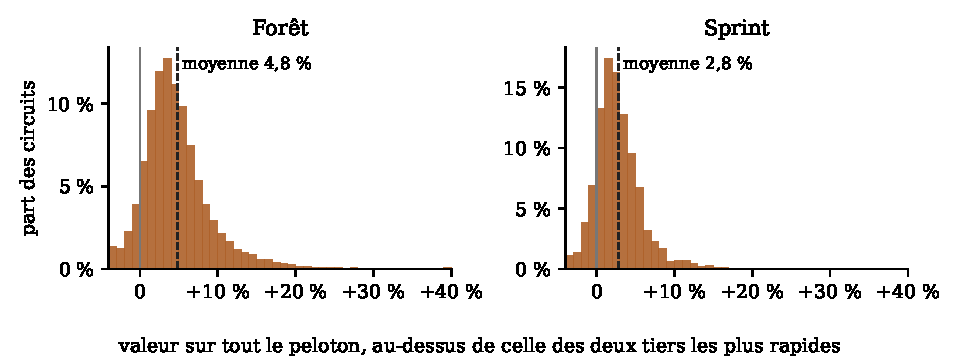
\includegraphics{fig_trunc.pdf}
\caption{Pour chaque circuit, de 2012 à 2026 : de combien la valeur mesurée sur tout le peloton dépasse celle des deux tiers les plus rapides.}\label{fig:trunc}\end{figure}

La part a été réglée dans chaque spécialité par un seul critère : celle qui prédit le mieux les duels de 2012 à 2024, sans perte significative depuis juillet 2025 (figure~\ref{fig:share}).
\begin{itemize}
  \item \textbf{Forêt : 90~\%.} Tout le peloton gagne \NallVsTwoF{} point sur les deux tiers, et 90~\% encore \NnineVsAll{} sur tout le peloton (\NnineVsAllN{} sur les courses nationales), mieux dans \NnineBetter{} saisons sur 15 et moins bien dans \NnineWorse. Le dernier dixième, ce sont les courses très perdues : les laisser de côté évite qu'un seul coureur égaré porte la valeur du circuit.
  \item \textbf{Sprint : les deux tiers}, la règle de la FFCO. Rien ne fait mieux sur les quinze saisons ; tout le peloton fait \NallVsTwoS. Les erreurs y sont deux fois plus rares qu'en forêt.
  \item \textbf{VTT : 75~\%} (\NvttSeventyFive). 85~\% fait le mieux de 2012 à 2024 (\NvttEightyFive), mais perd depuis juillet 2025 (\NvttEightyFiveT). \textbf{Ski : 75~\%}, comme le VTT : il a trop peu de courses pour être mesuré.
\end{itemize}

\begin{figure}[h]\centering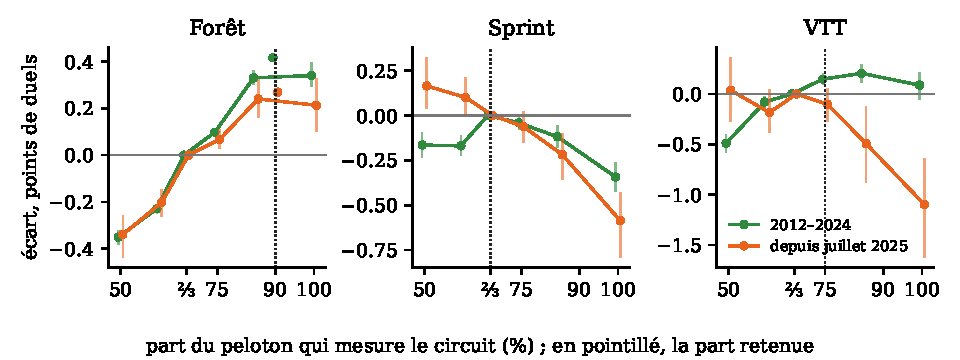
\includegraphics{fig_share.pdf}
\caption{Écart de la part des duels bien prédits face aux deux tiers les plus rapides, en points, selon la part du peloton qui mesure le circuit, avec l'intervalle à 95~\%. En forêt, le point à 90~\% est mesuré face à tout le peloton.}\label{fig:share}\end{figure}

\paragraph{La variante géométrique : une méthode empirique, étudiée pour ses performances.} Le « Top géométrique » est une autre façon de calculer le score \Top, étudiée du 7 au 16 octobre 2026 et publiée sur le site du 13 au 16 octobre. Il garde tout le reste de la méthode (les six places, les poids, le recalage) et change deux calculs.
\begin{itemize}
  \item \emph{La valeur du circuit, en moyenne géométrique.} Au lieu d'additionner les produits niveau habituel $\times$ temps puis de diviser par leur nombre, on les multiplie entre eux et on prend la racine : carrée pour deux produits, sixième pour six. Deux coureurs du même niveau, sur un circuit où ce niveau met d'ordinaire 60 minutes, courent l'un en 30 minutes, l'autre en 120 : la moyenne ordinaire de leurs temps vaut 75 minutes, leur moyenne géométrique $\sqrt{30 \times 120} = 60$ minutes. Le coureur deux fois trop lent et le coureur deux fois trop rapide s'annulent. S'y ajoute un réglage du poids des plus lents propre à chaque spécialité : tout le peloton en forêt, presque seulement les deux tiers les plus rapides en sprint, un intermédiaire en VTT et en ski.
  \item \emph{Le niveau habituel, en moyenne cubique.} On élève chaque score au cube, on fait la moyenne des cubes, puis on en prend la racine cubique. Pour 6\,000, 5\,000 et 4\,000, la moyenne ordinaire vaut 5\,000 et la moyenne cubique 5\,130 : elle penche vers les bonnes courses, sans écarter les autres.
\end{itemize}
Ces choix n'ont pas été posés à l'avance. Seule la moyenne géométrique a une raison simple : les temps se comparent en proportion. Le reste a été trouvé dans les données : la puissance de la moyenne, la part du peloton et le réglage de chaque spécialité ont été recalculés sur quinze saisons, plusieurs dizaines de variantes au total, et gardés parce qu'ils prédisaient mieux les duels. Le réglage du poids des plus lents vaut ainsi 0 en forêt et 400 en sprint sans qu'on sache dire pourquoi. C'est ce qui faisait l'intérêt de la méthode, étudiée pour ses performances, et sa limite : une règle qu'on ne peut ni justifier simplement, ni refaire à la main.

Face à elle, la méthode retenue fait, de 2012 à 2024 : \NgeoF{} point de duels en forêt (\NgeoNF{} sur les courses nationales), \NgeoS{} en sprint, \NgeoVTT{} en VTT. Ces écarts valent un ou deux duels sur mille : aucun coureur ne les verrait dans un classement, mais chacun verrait une règle plus difficile. La variante reste calculée sur le site, sous le nom « Top géométrique », pour comparaison.

Ce que la variante apprenait reste vrai : c'est la part du peloton qui mesure le circuit qui faisait la différence. En forêt, presque tout le peloton gagne près d'un demi-point sur les deux tiers, quelle que soit la moyenne.

\paragraph{Les courses des jeunes (19 octobre 2026).} Le \CN{} d'un jeune retarde sur son niveau : un an et demi plus tard, le niveau habituel d'un jeune a monté de 22~\% en forêt, celui d'un adulte de 11~\% (la montée générale de l'échelle comprise). Ses courses d'il y a dix mois décrivent un coureur plus lent. Une course courue en catégorie jeune (H et D jusqu'à 20 ans) compte donc dans la moyenne pour $1 - \text{âge} / \text{fenêtre}$ : en entier le jour de la course, à moitié six mois plus tard, presque plus à la fin de la fenêtre. Elle garde ses places ; les courses des adultes gardent leur poids ; la règle s'applique au niveau habituel, qui mesure les circuits, comme au \CN{} \Top. Le \CN{} de chaque règle a été relu le jour même, quinze jours avant chaque course.
\begin{itemize}
  \item \textbf{Forêt} : \NjunF{} point de 2012 à 2024, mieux dans \NjunFBetter{} saisons sur 15, \NjunFT{} depuis juillet 2025.
  \item \textbf{Sprint} : \NjunS{} de 2012 à 2024, rien de significatif depuis juillet 2025 (\NjunST).
  \item \textbf{VTT} : \NjunV{} de 2012 à 2024, \NjunVT{} depuis juillet 2025.
\end{itemize}
Faire vieillir les courses de tous les coureurs apporte peu : au mieux \NjunAdult{} en forêt (le poids divisé par deux tous les six mois), et rien de plus une fois les courses des jeunes effacées (\NjunBoth{} avec les deux). Le niveau d'un adulte bouge peu d'une saison à l'autre. Une fenêtre de deux ans fait \NjunWin{} ; effacer les courses dans le \CN{} \Top{} seul, sans toucher au niveau habituel, \NjunTop. Le prix : en forêt, les jeunes sont un peu plus souvent annoncés devant les H/D\,21--34 qu'ils ne finissent devant (\NjunBiasBefore{} points avant, \NjunBiasAfter{} après) ; en sprint et en VTT, où ils étaient sous-évalués, l'écart se réduit. Le \CN{} d'un jeune peut désormais bouger entre deux courses.

\paragraph{Les coureurs loin de leur niveau (18 octobre 2026).} Sur un circuit, quelques coureurs finissent loin de ce que leur niveau habituel laisse prévoir : bien plus vite, souvent des jeunes en progrès dont le niveau était en effet trop bas (un an plus tard, 17 à 19~\% au-dessus des autres coureurs de leur âge), ou bien plus lentement, après une erreur. 28 règles ont essayé de les écarter de la valeur du circuit : d'un côté ou des deux, au-delà d'un seuil ou en part fixe, et de ne plus laisser les jeunes mesurer les circuits. N'écarter que les plus rapides fait monter les circuits des jeunes, donc leurs \CN, donc la mesure de leurs circuits suivants : en forêt, leurs circuits finissent jusqu'à \NoutLoop~\% au-dessus de ceux des adultes, et la prédiction recule (\NoutFast, \NoutFastFive{} au seuil de 5~\%). Écarter les deux côtés coûte en forêt (\NoutBothF) ; en sprint et en VTT, ajouté à l'écart des jeunes, il gagne \NoutXS{} et \NoutXV. Ces gains demanderaient deux règles de plus dans la mesure des circuits, pour corriger le même défaut que l'effacement des courses des jeunes : un \CN{} de jeune en retard sur son niveau. La méthode garde la mesure des circuits telle quelle et traite ce retard là où il naît, dans le \CN.

\paragraph{Le recalage.} Le \CN{} d'un coureur est fait de ses meilleures courses, donc un peu au-dessus de ses courses ordinaires ; les circuits suivants sont mesurés avec ces niveaux un peu hauts, et le niveau général monte de quelques dixièmes de pour cent par mois. Le facteur d'un jour était calculé sur un niveau qui avait 18 à 20 mois de retard, et le niveau publié dépassait la cible de 7~\% en forêt. Prolonger la moyenne de 13 mois au rythme de la montée des dix dernières années garde un facteur aussi régulier, et ramène le niveau publié près de la cible : depuis 2018, à 2~\% en moyenne en forêt et en VTT, à 3~\% en sprint, avec des écarts de 6 à 9~\% après les saisons Covid.

\paragraph{Les autres idées.} Chaque idée a été recalculée et jugée de la même façon ; aucune n'a été retenue.
\begin{itemize}
  \item \emph{Rendre le retard plus cher}, en élevant le temps à une puissance : c'était en fait changer les moyennes du circuit et du \CN{} ; la moyenne quadratique, en ligne du 7 au 13 octobre, bousculait les classements sans corriger la part du peloton.
  \item \emph{Une règle temps-score propre à chaque circuit} : moins bien ; sur une vingtaine de coureurs, l'estimation est trop incertaine.
  \item \emph{Plus de poids aux courses qui départagent mieux les coureurs} : pas de différence significative.
  \item \emph{Un score qui pénalise moins les très grosses pertes de temps} : un peu mieux en forêt, nettement moins bien en sprint.
  \item \emph{Le niveau estimé par un modèle statistique} qui sépare la forme du jour et les erreurs : \NmleS{} point en sprint, \NmleF{} en forêt, où se tromper souvent est un trait du coureur.
  \item \emph{Atténuer les temps aberrants} (méthode de Huber) au lieu de régler la part du peloton : environ 0,1 point de moins.
  \item \emph{Une valeur de circuit commune aux circuits de même longueur en sprint}, \emph{un score fondé sur l'écart au temps moyen} à la façon de l'IOF, \emph{un recalage qui réagit à ses propres effets} : moins bien, ou instable.
\end{itemize}

\section{Résultats}

Sur les saisons 2012 à 2024, qui n'ont pas servi aux réglages, et sur les mêmes coureurs :
\begin{center}\small
\begin{tabular}{@{}lrrrr@{}}\toprule
 & \multicolumn{2}{c}{Forêt} & \multicolumn{2}{c}{Sprint} \\
 & officiel & \Top & officiel & \Top \\ \midrule
duels bien prédits & \NaccFoff~\% & \NaccFtop~\% & \NaccSoff~\% & \NaccStop~\% \\
écarts de temps expliqués & \NrrFoff~\% & \NrrFtop~\% & \NrrSoff~\% & \NrrStop~\% \\ \midrule
gain du \Top{} en duels, toutes les courses & \multicolumn{2}{c}{\NgainF} & \multicolumn{2}{c}{\NgainS} \\
gain du \Top{} en duels, courses nationales & \multicolumn{2}{c}{\NgainNF} & \multicolumn{2}{c}{\NgainNS} \\
gain du \Top{} en écarts de temps expliqués & \multicolumn{2}{c}{\NgainRF} & \multicolumn{2}{c}{\NgainRS} \\
saisons où le gain est significatif & \multicolumn{2}{c}{\NwinsF} & \multicolumn{2}{c}{\NwinsS} \\ \bottomrule
\end{tabular}
\end{center}
Ces chiffres portent sur \NcompsF{} compétitions de forêt et \NcompsS{} de sprint, chaque circuit pesant son nombre de coureurs ; les gains sont en points, avec leur intervalle à 95~\%. Les jeunes, que le \CN{} officiel sous-évalue de \NcalibYoungOff~\% en forêt face aux H/D\,21 (leurs circuits provoquent beaucoup d'erreurs), étaient à leur place quand tout le peloton mesurait le circuit (étude du 13 octobre). Les vétérans restent surévalués de 8 à 9~\% par toutes les méthodes, la méthode officielle comprise : la cause n'est pas la mesure du circuit.

\section{Conclusion : la plus simple de celles qui prédisent le mieux}

Toutes les variantes essayées se tiennent en quelques dixièmes de point de duels bien prédits, et les meilleures en quelques centièmes. À ce niveau, un gain ne se voit plus dans un classement, mais une règle compliquée se voit dans chaque explication. La méthode retenue garde donc le score de la FFCO et des moyennes ordinaires, et ne change que ce qui compte vraiment : les meilleures courses retenues sur six places, une part du peloton réglée par spécialité pour mesurer les circuits — 90~\% en forêt, les deux tiers en sprint, 75~\% en VTT et en ski —, un recalage continu, et des courses de jeunes qui comptent de moins en moins avec le temps. Elle gagne plus de deux points de duels sur le \CN{} officiel, en forêt comme en sprint ; depuis que les courses des jeunes s'effacent avec le temps, elle fait mieux en forêt que la variante géométrique qui l'a précédée, et jeu égal en sprint.

Cette méthode est en ligne depuis le 16 octobre 2026 sur O'CN, sous le nom « Top » ; les courses des jeunes y comptent de moins en moins avec le temps depuis le 19 octobre. Le classement officiel y reste la seule référence qui fait foi. Les données proviennent du site du classement national de la FFCO : une course absente, mal saisie ou corrigée ensuite peut expliquer un écart. Les méthodes calculées par le site partent des \CN{} de 2010, et leurs premiers mois reflètent surtout ce point de départ.

\end{document}
